\begin{figure}[t]
  \centering
  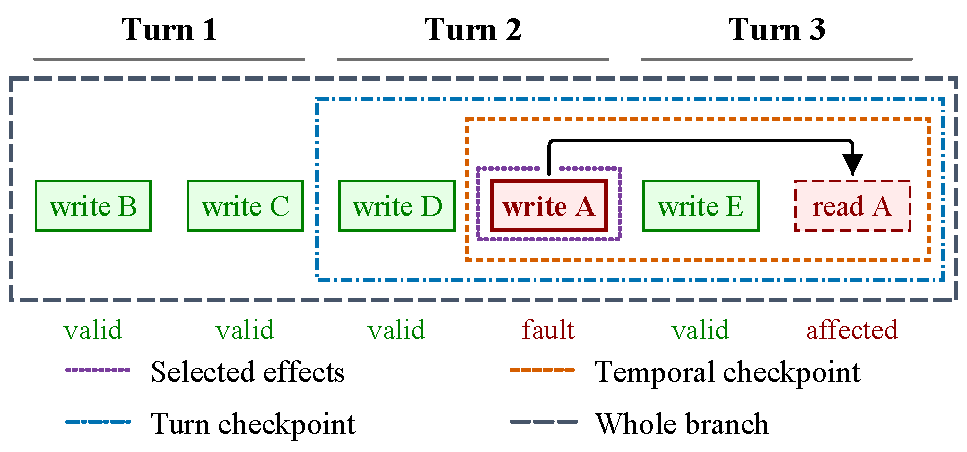
\includegraphics[width=\linewidth]{figures/recovery-granularity/FIG-Recovery-Granularity.pdf}
  \caption{\textbf{Recovery granularity of existing approaches.}
  Six calls execute across three turns. Red calls are faulty or affected;
  green calls are independent. Four outline styles mark the selected
  invocation effects, temporal suffix, turn-boundary suffix, and whole
  branch. The arrow denotes dependency; effect selection alone leaves
  the later read affected.}
  \label{fig:recovery-granularity}
\end{figure}
